% !TeX spellcheck = en_GB
% !TeX root = Report.tex
\phantomsection
\addcontentsline{toc}{subsection}{Lecture 1 - Fabrice Perrot, Alstom}
\subsect{Lecture 1 - Fabrice Perrot, Managing Director Alstom Grid Research and Technology Centre}
Alstom Grid is one of four technology sectors making up the Alstom group including transport, thermal power and renewable energy. 
The grid sector was formed in 2010 when Alstom acquired Areva's transmission and distribution arm \cite{AlstomGridInfo} for \euro2.3bn \cite{AlstomAreva}. 
With a worldwide presence and over 20,000 employees \cite{AlstomGridInfo} the company delivers a large number of services and products for the HV grid sector.
Projects undertaken can be very large scale, including a \euro62m involvement in floating substations in the German north sea \cite{AlstomGridInfo}, building the Gulf's largest High Voltage Direct Current (HVDC) converter station \cite{AlstomGulf}, and delivering the converter transformers for the world's longest HVDC transmission scheme at Rio Madeira in Brazil \cite{AlstomRio}.

\begin{figure}[!h]
\centering
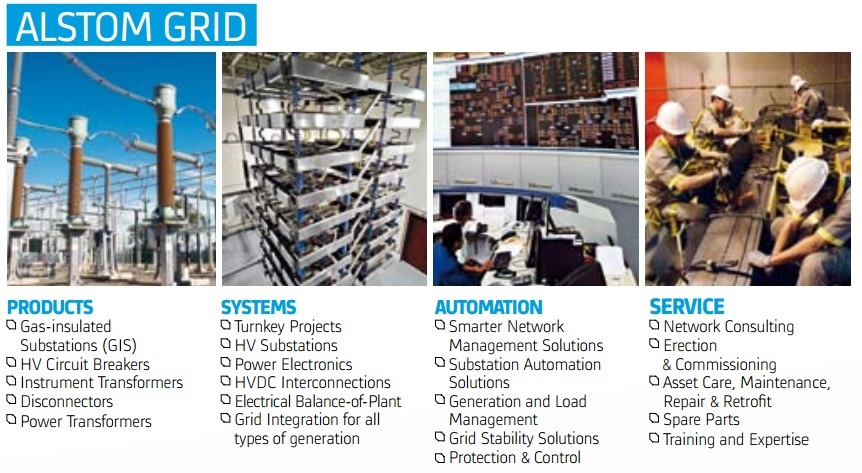
\includegraphics[width = 0.7\textwidth]{Figures/AlstomGrid.jpg}
\caption{Alstom Grid Services - reprinted from \cite{AlstomGridInfo}}
\label{figure:AlstomGrid}
\end{figure}

The electrical transmission and distribution infrastructure is an often overlooked service critical to maintaining a western lifestyle.
The supergrid infrastructure in the UK was largely built in the 1950s to cater for the connection of the large coal and gas power stations to the large load centres \cite{NationalGrid75}.
The nature of the electricity industry is fundamentally changing, an increase in embedded generation and the increased remoteness of renewable sources means the infrastructure is no longer fit for purpose, with a significant investment required.

The renewable drive in the energy industry is driven by government policy.
The Climate Change Act 2008 sets out the target to reduce carbon emissions by 80\% of 1990 levels by 2050 \cite{ClimateChangeAct08}.
In order to meet this commitment in any meaningful sense, the electricity sector must be decarbonised considerably earlier than 2050, so that space heating and transport sectors can transition to a carbon-neutral energy vector.
There is a unified approach in many developed nations, particularly in Europe, promoting renewable energy development.
It is this legislation that is driving the change in the design basis for almost all modern transmission and distribution infrastructure.

The opportunities to profit from developing and installing this infrastructure is huge.
In the UK, the cost of reinforcements is estimated at \pounds8.8bn \cite{NetworkStrategyGroup}. 
The study estimates that a large majority of the investment will be required for the connection of on and offshore wind, usually by HVDC links where appropriate.
Opportunities for this type of large infrastructure project are at a global scale, and include developed and developing nations.
Another opportunity of note is the DeserTec solar project, with the aim of connecting the North African grid to the European Super Grid providing access to cheap, carbon-free concentrating solar power plants. 
The project is an extremely challenging endeavour considering the political cooperation involved, but should the project ever proceed, the investment could total \$560bn \cite{DesertTec}.

\begin{figure}[!h]
\centering
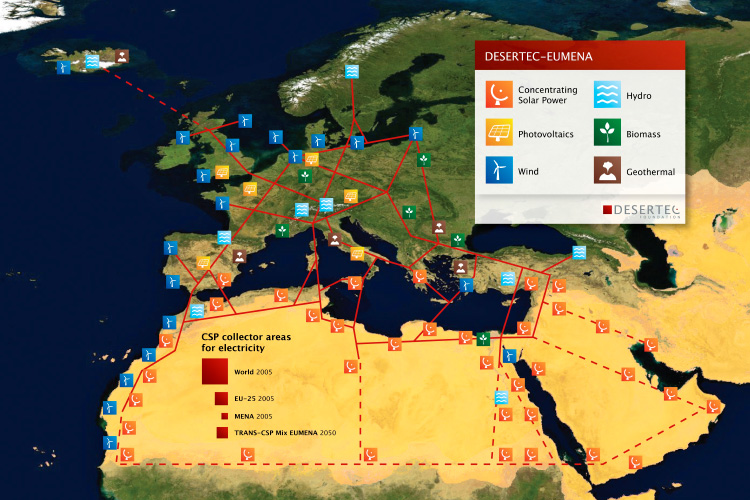
\includegraphics[width = 0.7\textwidth]{Figures/Desertec.jpg}
\caption{Potential structure of the DeserTec HVDC network extending over the Middle East, North Africa and Europe - reprinted from \cite{DesertTec}}
\label{figure:Desertec}
\end{figure}

Considering these significant opportunities, Alstom's acquisition of Areva Transmission and Distribution seems a clever strategic investment.
The acquisition of a core competence in HVDC and other grid services and technologies at a time when global government policy is promoting renewed investment in the sector is clearly an attempt to align with the opportunities provided by emerging Government policy.





